\documentclass[conference, compsoc, onecolumn]{IEEEtran}
\IEEEoverridecommandlockouts
% The preceding line is only needed to identify funding in the first footnote. If that is unneeded, please comment it out.
\usepackage{cite}
\usepackage{amsmath,amssymb,amsfonts}
\usepackage{algorithmic}
\usepackage{graphicx}
\usepackage{textcomp}
\usepackage{xcolor}
\usepackage{subfigure}
\usepackage{float}
\usepackage{color,soul}

\def\BibTeX{{\rm B\kern-.05em{\sc i\kern-.025em b}\kern-.08em
    T\kern-.1667em\lower.7ex\hbox{E}\kern-.125emX}}
\begin{document}

\renewcommand\thesection{\arabic{section}}
\newcommand\norm[1]{\left\lVert#1\right\rVert}

\graphicspath{ {./figures/} }

\title{SYSC5804 Project: MIMO Channel Reconstruction\\
{\footnotesize Prepared for Dr. Jun (Steed) Huang}

}

\author{\IEEEauthorblockN{James Baak}
\IEEEauthorblockA{{Department of Systems and Computer Engineering} \\
\textit{Carleton University}\\
Ottawa, Ontario \\
JamesBaak@cmail.carleton.ca\\
101002918}
\and
\IEEEauthorblockN{Ben Earle}
\IEEEauthorblockA{{Department of Systems and Computer Engineering} \\
\textit{Carleton University}\\
Ottawa, Ontario \\
BenEarle@cmail.carleton.ca\\
100970237}
}

\maketitle

\begin{abstract}
Reducing feedback and overhead for channel reconstruction in massive Multi-Input Multi-Output (m-MIMO) systems is an active problem in 5G wireless research \cite{Ye2018}. This report documents the author's SYSC5804 term project, implementing state-of-the-art channel reconstruction techniques and exploring new methods to reducing run-time, and/or increase accuracy. Two existing methods were implemented: the first is a regression based approach, using an algorithm called Least Absolute  Shrinkage  and  Selection  Operator (LASSO) \cite{Han2019}; the second transformed the received pilots into an image and used deep learning image processing algorithm You Only Look Once (YOLO) to extract path information \cite{Li2020}. Additionally, a new method is implemented using autokeras \cite{jin2019} to build and train a Deep Neural Network (DNN) to predict the path information directly from the channel images. The authors present the results of each approach, implementation challenges, and future work. All the code referenced in this report is available on GitHub \cite{git}.

\end{abstract}

\begin{IEEEkeywords}
Channel Reconstruction, 5G, Simulation, Neural Networks
\end{IEEEkeywords}

\section{Introduction}
Telecommunication systems demand constant innovation, and the requirements grow exponentially with each generation of the wireless technology. One of the ways the 5th Generation (5G) wireless systems respond to these growing requirements is using massive Multi-Input Multi-Output (m-MIMO) antennas \cite{Dahlman2018}. These systems have the potential to improve the channel bandwidth, coverage, and capacity through beamforming and spatial multiplexing. To take advantage of these perks, the systems require accurate Channel State Information (CSI), which are metrics that describe how the channel will affect the signal. However, increasing the number of antennas increases the complexity and overhead when measuring the CSI, known as channel sounding \cite{Mawatwal2020}. These computations are built using a matrix of complex numbers, called the channel matrix, in which each element includes a gain and angle which, when multiplied by the transmitted signal will estimate the received signal (without any noise). The channel matrix grows exponentially with the addition of new antennas, further complicating channel reconstruction algorithms that try to rebuild the channel matrix based on CSI and/or received pilots. Classical algorithms will fail to meet the real-time constraints in these massive antenna systems \cite{Li2020}.

Machine Learning (ML) is an increasingly popular approach for improving the accuracy, feedback overhead, and runtime of channel reconstruction \cite{Ye2018}. 5G wireless communication systems are complex, making it difficult to implement and maintain new algorithms. Additionally, classical algorithms such as those described in \cite{Han2019} and \cite{Liu2016} have very high computational complexity. Alternatively, data-driven models eliminate the analytical complexity in the conventional methods above. ML can easily identify trends in multi-dimensional data in ways that humans cannot. Although, training a model is computationally taxing and requires a lot of data, once the model has been trained, it is very fast to execute \cite{Li2020}. ML solutions are often faster to execute and with equivalent performance, if not better, than existing solutions. 

Through this term project the authors explore channel reconstruction with simulated data. The data was generated using a simulator built with the MATLAB 5G Toolbox \cite{matlab2020}. State of the art channel reconstruction techniques were recreated using MATLAB and Python. These methods include using Least Absolute Shrinkage and Selection Operator (LASSO) \cite{Han2019} and image processing technique You Only Look Once (YOLO) \cite{Li2020}. Furthermore, the authors experimented with applying Deep Neural Network to the channel directly to predict the path gains, angles and delays. The remainder of this paper is organized as follows. First, the background section defines the wireless concepts required for this work, the existing channel reconstruction algorithms, and machine learning algorithms used. Section 3 documents the simulator and the 5G Toolbox functions used. Section 4 will explain the image generation process, along with the available configuration for the channel models Section 5-7 describes the implementation, results and challenges faced with the YOLO, LASSO, and DNN methods, respectively. Finally, Section 8 concludes the paper.  

\section{Background} \label{background}
This section will describe the wireless communication and machine learning concepts involved in this work at a high level. The section starts with wireless channels, channel sounding and channel reconstruction. Then the section provides background to the algorithms used for channel reconstruction: LASSO, YOLO, and DNNs.  

\subsection{Wireless Concepts}
The wireless channel is the physical medium traversed by the signal. The channel is described mathematically by a matrix of complex numbers, H. The received signal \(\textbf{Y}\), is related to the transmitted signal as follows, \(\textbf{Y} = \textbf{H} \textbf{S} + \textbf{Z} \). Where \(\textbf{S}\) is the transmitted signal and \(\textbf{Z}\) is additive white gausian noise. The goal of this work is to reconstruct the channel matrix \(\textbf{H}\), from the received signal \(\textbf{Y}\). The remainder of this subsection will define key concepts: channel sounding, channel reconstruction from paths, channel reciprocity, and channel sparsity.
\subsubsection{Channel Sounding}
Radio systems require knowledge of the channel they will be transmitting over to optimize the communication. Important decisions are made with this information, such as the modulation scheme or the beamforming precoding matrix. For instance, lower SNR channels can support more bits per symbol, increasing the channel's throughput. However, if the channel cannot support the modulation scheme chosen then the bit error rate will be so high that the signal cannot be recovered. Channel sounding is done by transmitting a reference signal over the channel. The reference signal contains pilot symbols known to both the transmitter and the receiver. The receiver uses the difference between the received signal and the expected signal to estimate the channel conditions. Using these estimates the system will calculate CSI metrics such as the Channel Quality Indicator (CQI), Received Signal Strength Indicator (RSSI), Precoding Matrix Indicator (PMI), and Rank Indicator (RI) \cite{Dahlman2018}. CQI is an integer index into a list of Signal to Noise Ratio (SNR); there are 15 values, the higher the CQI, the better the SNR. RSSI simply returns the signal power measured at the receiver in negative dB, it typically ranges from 0-127. PMI is used in MIMO systems, it is an integer index into a list of potential precoding matrices. The matrix selected will be multiplied by the signals to be transmitted, mapping and scaling them for the appropriate antennas. Figure \ref{fig:pmibook} is an example of a simple PMI codebook. This code book is for two transmit antennas, with either one or two layers. Layer in this context is the number of symbols being transmitted at once. Rank Indicator (RI) is related to the rank of the channel matrix, if the RI is one then there is one independent path between transmitting antennas and receiving antennas. Therefore, the transmission is limited to being one layer. RI operates as the maximum number of supported layers. The highlighted square in figure \ref{fig:pmibook} is the precoder matrix for a PMI of 1 and a system configured to transmit 2 layers.

\begin{figure}[H]
    \centering
    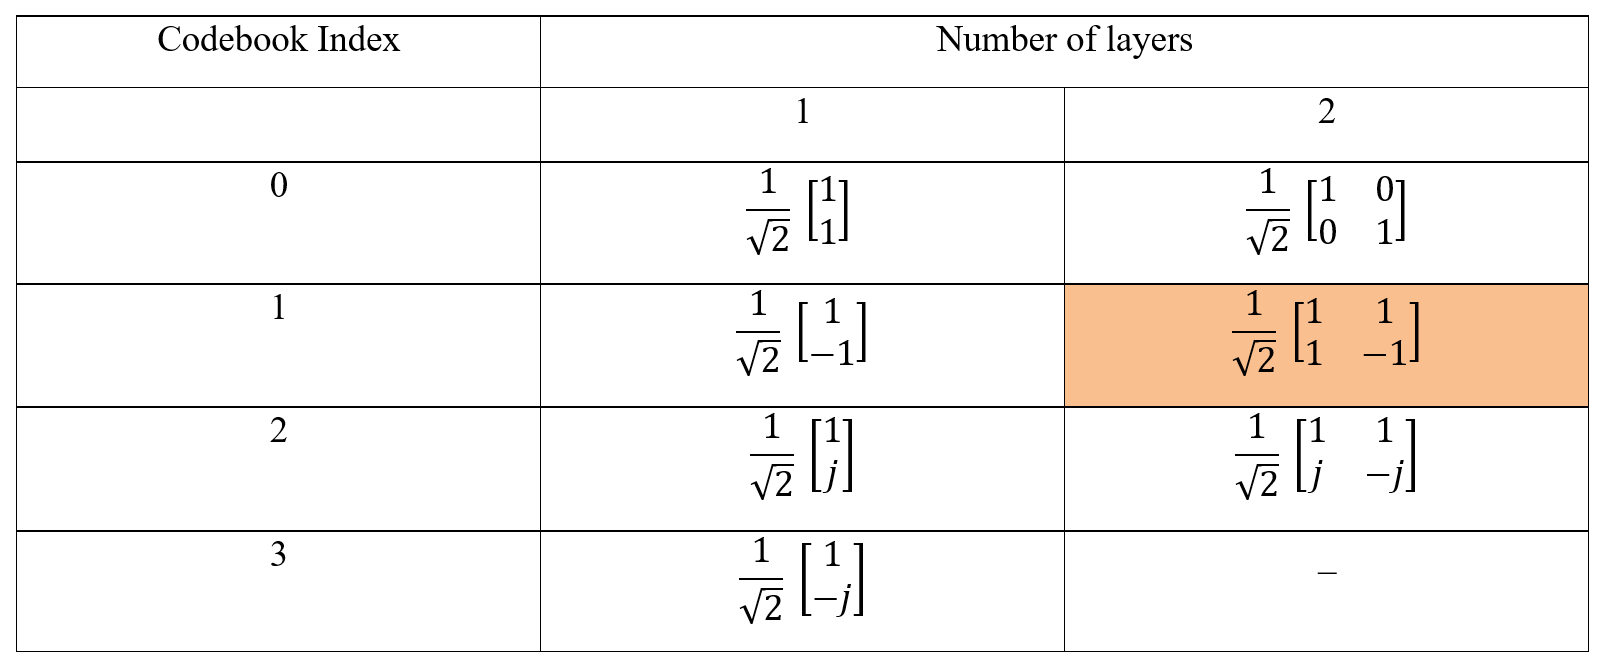
\includegraphics[width=15cm]{figures/PMI_Codebook.png}
    \caption{Example PMI Codebook \cite{Ryu2020}}
    \label{fig:pmibook}
\end{figure}

\subsubsection{Channel Reconstruction from Path Components} \label{sssec:chrec}

Wireless signals are impacted by objects in their path, causing them to experience reflection, refraction, and dispersion. Shadowing is the attenuation caused by obstacles in the path between the transmitter and receiver. Signals are not limited to following a single path to the receiver; often referred to as multipath effects. Each path will experience a different channel, as they may have different obstacles or distance. This will cause the signals to take a different amount of time to propagate to the receiver resulting in a different delay, phase, and gain for each of these paths. When adding signals that are out of phase they can either add constructively or destructively. Moving the receiver slightly can change the relative phase between signals causing a significant change in received power. Using knowledge of the path gains, angles, and delays the channel matrix can be reconstructed. The work done in \cite{Li2020} and \cite{Han2019} shows that the channel matrix is modeled with the following set of equations.
\[
    \textbf{h} = \sum_{l=0}^{L-1} g_{l} ( \textbf{p}_{l} (\tau) \otimes \textbf{a}(\theta_{l}) )
\]

\[
    \textbf{p}(\tau) = [e^{-j 2 \pi \frac{N}{2} \Delta f \tau}, ..., e^{-j 2 \pi (\frac{N}{2} - 1) \Delta f \tau}]
\]

\[
    \textbf{a}(\theta) = [e^{-j 2 \pi \frac{M}{2} \frac{d}{\lambda} \mathrm{sin}\theta}, ..., e^{-j 2 \pi (\frac{M}{2} - 1) \frac{d}{\lambda} \mathrm{sin}\theta}]
\]

\noindent
Note that \([\cdot]^{H}\) is the Hermitian Transform (complex conjugate transpose) and \(\otimes\) is the Kronecker Product. L is the number of paths. The individual path parameters \(g_l\), \(\tau_l\), and \(\theta_l\) are the gain, delay, and angle of the \(l^{th}\) path, respectively. Furthermore, \(\textbf{p}(\tau)\)and \textbf{a}\((\theta)\) are the delay-related phase vector and steering vector of a Uniform Linear Array (ULA) of antennas, respectively. All the remaining variables are constants chosen for a given communication system; \(d\) is the distance between antennas, \(\lambda\) is the carrier wavelength, and \(\Delta f\) is the carrier sub-spacing. This set of equations will be used to reconstruct the channel matrix after predicting the path components.

\subsubsection{Channel Reciprocity}
One of the main advantages to Time Division Duplexing (TDD) is that the uplink and downlink channels are the same; this is known as channel reciprocity. Alternatively, Frequency Division Duplexing (FDD) channels will experience frequency specific channel effects. This requires FDD systems to do channel sounding in both the uplink and downlink directions, then feed the results back over the channel. TDD can skip the channel sounding feedback step since it knows the channel is the same etiher way. This feedback step has very high overhead, especially in m-MIMO systems. The previously mention channel reconstruction technique is advantageous because the all the path parameters are frequency independent with the exception of the gain. This means the uplink and downlink values will be the same, even in an FDD system. Therefore, using this channel reconstruction scheme, the only feedback needed is to tune the path gains \cite{Han2019}. 

\subsubsection{Channel Sparsity}
In FDD m-MIMO systems the concept of channel sparsity is quite important and is exploited in many channel sounding techniques, such as LASSO and Netwonized Orthogonal Matching Pursuit (NOMP). Sparsity simplifies the problem of finding a channel's characteristics. In the context of this report, channel sparsity is the spatial channel sparsity for a channel vector and assumes there is a finite number of paths for downlink communication between a Base-Station (BS) and it's User Equipment (UE). Channel sparsity exists due the local scattering effects at the BS's antennas, and the temporal and spatial limitations of the signal paths available for a particular user time due to factors like interference \cite{Liu2016}. As the number of antennas in our m-MIMO system increases the scattering effect is amplified and the available paths for a UE becomes more limited. Therefore, the desired channel vector can be estimated using techniques that take advantage of the sparse channel vector structure.

\subsection{Deep Neural Networks}

Deep Neural Networks (DNN) play an important role in our project as one of the project objectives was to explore deep learning methods for downlink channel reconstruction for m-MIMO systems.  DNN and deep learning involve using multi-layered neural networks using several different techniques, such as Convolution Neural Networks (CNN), skip connections, and residual neural networks \cite{Burkov2019}. The number of layers for a deep learning network can vary, but generally contains more than one hidden layer.
Convolution Neural Networks are machine learning models which contain convolution layers. Convolution layers consist of weighted filters that are applied over a large input matrix which usually originated from a image or video source \cite{Burkov2019}. CNNs were invented for image and video processing with applications of object detection and classification in mind. CNNs have important roots in problem areas such as autonomous vehicles. In our project, CNNs were employed in YOLO's object detection, more in the subsequent subsection.

\subsection{YOLO}

You Only Look Once (YOLO) are a series of real-time object detection models developed for coloured images with complex classification targets. With real-time requirements for video detection, the model is very quick due to the fact that an image is processed with one pass of the deep network \cite{Redmon2018}. YOLO works differently than other object detectors which use classifiers or localizers to locate potential targets within an image and then run the model over different section of the image at three different scales. Running the detection process at three different scales enables YOLO to also detect objects that are of smaller size in an image, making it an ideal candidate for the detection of the small path objects discussed in Section \ref{image-gen}. YOLO passes the whole image through the detection model giving it an advantage of run-time speed and also the ability to take into account the global context of the whole image. YOLO's network structure can be split into three parts for the proposes of the report; the input layer, the hidden layers, and the output layers.

The input layer of YOLO takes a compressed version of an image to run detection over before delivery to the first CNN in the hidden layers. Compression of the image is very common in deep learning in order to lower the complexity of the model and also improve training and run-time. The input layer specifies three values which define the required image input size. The parameters are image width, height, and number of channels. Width and height describe the image size while the number of channels represent the values for each pixel. A grayscale image will have only one channel while a common RGB image has three channels. YOLO's pretrained models available for transfer learning use three channels to process RGB images, so any grayscale images must be preprocessed before the YOLO model can be used.

The hidden layer of YOLO changes depending on the version of YOLO in use. YOLOv2 uses Darknet-19, while YOLOv3 uses Darknet-52 \cite{Redmon2018}. The exact YOLO hidden network architecture can be substituted though with other network structures that preform well in objection detection such as ResNet-50 \cite{Matlab2021a}. The hidden layer provides the backbone for the object detection network and is where most of the training of our model's weights will occur. Darknet is an open-source neural network framework written for deep neural network design. As mentioned above, Darknet was used in the construction of both YOLOv2 and YOLOv3 and their training. Having the flexibility to change the network structure is quite important so that the network can adapt to the specific application. This flexibility also enables the construction of networks with varying hidden layer designs. In the case of our project, we did not need to take advantage of all 53 convolution layers of Darknet-53 because we believe the images that we are processing are much more simple than a complex RGB image with many different shapes and objects within the image. The images produced only have one class and has an object shape that is quite consistent making picking up the object with the CNN much easier. More on this in Section \ref{yolo-main} when model tuning is discussed.

The last part of the YOLO model are the output layers. For the process of object detection to be complete the output from the last or one of the convolution layers is taken and transformed into a series of anchor boxes that are uniformly distributed across the image data. These boxes represent the regions of interest in the image and each box predicts the probability of a target object lying within. The transform layer connects the output of the chosen convolution layer and the final output layer and evaluates the initial anchor boxes. The final output layer refines the predictions and anchor boxes from the previous transform layer producing the final output \cite{Matlab2021a}. 

When the three parts of the YOLO network model are combined, a preprocessed image can be given to the model to predict the location and bounds of target objects within the image. A threshold is used to determine which anchor boxes of the detector are valid and which are false positives. Therefore the threshold can be viewed as a hyperparameter for tuning the network detection of objects within the image. It is especially handy for our project's application since there is only one class of object of interest. This means that the threshold can be lower than normal to ensure all channel paths within an image are gathered. By default the threshold of object detection models in MATLAB is 0.5, but can be easily modified for different applications.

\subsection{LASSO} \label{lasso-back}

Least Absolute Shrinkage and Selection Operator (LASSO) is a linear regression technique that shrinks the absolute prediction error and is accompanied with a tuning parameter $\lambda$ which defines the minimum value of the sum of the regression coefficients \cite{Ranstam2018}. LASSO is a type of L1 regularization method since it contains an added penalty parameter to reduce the number of coefficients within the weights \cite{Ranstam2018,Tibshirani2013}. This type of regularization can be very useful for activities such as feature selection and models that have sparse structures such as the channel sparsity in FDD m-MIMO systems. LASSO can be represented mathematically using the following definition:

\[ \min_{\beta} \norm{y - x\beta}^2_2 + \lambda |\beta|_1 \]

Where \(y \in \mathbb{R}^{M \times 1}\),  \(x \in \mathbb{R}^{M \times N}\), \(\beta \in \mathbb{R}^{N \times 1}\), and \( { \lambda \in \mathbb{R} | \lambda \geq 0 } \). $x$ defines our $M \times N$ input matrix and $\beta$ are the unknown coefficients applied to the matrix to generate the output vector $y$. LASSO regression will minimize or eliminate the coefficients in the $\beta$ vector to satisfy the equation above. Setting $\lambda = 0 $ will just perform normal linear regression as the penalty proportion would go to zero. Increasing the value of $\lambda$ will increase the sparsity of the $\beta$ vector by setting more and more of the values in $\beta$ to zero.

As described in the paragraph above, the LASSO regression functions on real valued matrices and vectors whereas in the application of channel reconstruction, the values used to represent the channel vector and signals are complex values ($H,x,y \in \mathbb{C}$, where H, x, and y are the channel vector, transmitted signal, and received signal respectively) \cite{Liu2016}. To overcome this complication, the normal LASSO regression function defined in MATLAB has to be modified or another LASSO function has to be imported to handle the complex values of the channel model's representation. Both methods were used in this project and are discussed more in Section \ref{lasso-main}.


\subsection{NOMP}
Matching Pursuit (MP) is an algorithm used for compressed sensing, which leverages the sparsity of a signal to represent it with far fewer measurements than otherwise possible. The MP algorithm uses an over complete dictionary of functions and a vector of weights to scale each function. Then the algorithm estimates the function as the vector of weights multiplied by the dictionary of functions. The algorithm uses a greedy optimization scheme to quickly find a solution to the weight vector. At a high level, the algorithm is similar to a Fourier series analysis if the dictionary of functions were to be a set of all sinusoidal functions. The Orthogonal MP (OMP) is an extension improves the accuracy of the prediction while adding computational complexity. Furthermore the Newtonized OMP adds a refinement step to further improve the results. The authors in \cite{Han2019} use NOMP to reconstruct the channel by estimating the path gains, angles and delays. Implementing NOMP was considered for this project, as the clasical algorithm to compare the YOLO method with. However, due to its complexity LASSO was chosen in its place.




\section{Simulators} \label{sim}
All the channels were simulated in MATLAB using the 5G Toolbox. The MATLAB 5G toolbox provides a library of functions and examples for simulating the 5G NR wireless channels. This includes various physical layer models to simulate the functionality of the transmitter and receiver (e.g., modulation and encoding) as well as the different effects of the wireless channel. Figure \ref{fig:sim} shows the simulator's architecture.
\begin{figure}[H]
\centering
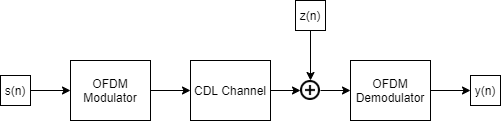
\includegraphics[width=15cm]{figures/SYSC5804-SimulationOverview.png}
\caption{Simulator Architecture}
\label{fig:sim}
\end{figure}
\noindent
The received pilots \textit{s(n)} are modulated with the 'nrOFDMModulate' modulate function. The carrier is configured to have a central frequency of 3.5GHz, a bandwidth of 90MHz, a sub-carrier spacing of 75kHz, and 32 transmit and receive antennas. These values were chosen to match those used in \cite{Li2020}. The number of antennas were varied, however most of the results were generated using 32 antennas since the resulting data sets were more manageable.  The modulated signal is passed through a 'nrCDLChannel' channel object with a custom delay profile. The CDL channel was chosen due to the configurable custom profile, it supports variable path count, gains, delays, angles, and angle spread. The simulator generates random CDL profiles for the channel model; this was used for generating diverse training data. The path count was limited to be significantly less then the number of antennas since most of the channel reconstruction algorithms required sparsity. After applying the channel effects the signal was subject to additive white Gaussian noise, $z(n)$. The noise power was a parameter of the simulation, different tests required different SNR. Finally, the signal was demodulated using 'nrOFDMDemodulate', resulting in $y(n)$, the received pilot symbols. 

The simulator aggregates the channel conditions and stores them in a CSV file along with a reference to the measurements done on the received pilots, such as the channel image discussed in the next section. The CSV has an entry for the each of the path gains, angles, and delays. The data set captures all the information needed to reconstruct the CDL channel used in the simulation. The only thing it does not capture is the noise power, antenna count and carrier details, which were typically held constant. This data set is used for training and testing the machine learning methods described in Section \ref{autodnn}.

The primary challenge faced while developing the simulator was the need for the modulation and demodulation functions. Both \cite{Li2020} and \cite{Han2019}, set all the received pilots to 1, shown mathematically, \(s(n) = 1, \forall n\) and attempted to pass these values through the channel directly. Neither paper discussed modulating the signal, so naively this step was skipped. The resulting received pilots made little sense and none of the algorithms were able to use them for channel reconstruction. For instance, the image generation held all the points against one axis, unable to move them in the angle space. After some research modulation was added to the simulator resolving these issues. 

A MATLAB script was made to test channel reconstruction from the ground truth values of the paths, it is available on GitHub titled "ChRecFromPaths.m" \cite{git}. The script simulated the wireless channel as previously described and used the received pilots without any noise as the ground truth value for the channel matrix. The equations described in \ref{sssec:chrec} were used along with the ground truth data for the paths to recreate the channel. The resulting estimated channel with a RMSE of 3.5e-05. This was considered acceptable accuracy, any error was most likely due to rounding in the floating point number math. The methods in this script would be used for channel reconstruction by the YOLO method, had the path components been properly calculated.

\section{LASSO} \label{lasso-main}
\subsection{Method and Implementation}
As described in Section \ref{lasso-back}, LASSO is a regression technique that finds weights applied to an input to produce a known output. This technique can also work on noisy outputs and thus can be applied to channel reconstruction of sparse channels. The channel is modeled in the form of:

\[ y = \Psi h + n \]

Where $y$ is the received signal, $\Psi$ is the transmitted reference signal containing the sequence of pilot symbols, $h$ is the channel vector and the main component used for channel reconstruction, and $n$ is the noise of the channel between two communicating entities \cite{Tse2004}. In the case of LASSO regression for channel sounding the transmitted and received reference signals can be converted into their angular domain representation using the Inverse Discrete Fourier Transform of the transmitted signal or by using the following transform from \cite{Tse2004}:

\[ \Psi^a = U_t \Psi \]

\[ U_t(k,l) = \dfrac{1}{\sqrt{n_t}} exp(\dfrac{-j2\pi k l}{n_t}) \] 

Where $n_t$ is the number of transmit antennas in our MIMO Uniform Linear Array (ULA) of antennas. $U_t$ is a unitary matrix that is $n_t \times n_t$, and $k$ and $l$ are the row and column indices of the square $U_t$ matrix \cite{Tse2004}. $U_t$ represents the matrix to preform the Inverse Discrete Fourier Transform on the transmitted signal $\Psi$ to yield the angular domain representation of the signal.

LASSO sends the reference signals from the MIMO BS station to the UE in evaluation to preform channel sounding. The UE will then send the compressed received reference signal back to the BS for further processing and channel estimation \cite{Liu2016}. This method is used for two main reasons. The first is to reconstruction the downlink channel between the BS and the UE, so the reference signal should be transmitted from the BS to the UE to estimate the downlink channel. Secondly, depending on the channel sounding technique used, the power and processing resources required to reconstruction the estimate of the channel vector can be expensive. This is especially impactful for wireless UE devices that run on batteries and have limited computing power or lack specific hardware to decrease the running times of the reconstruction techniques.

Using the CDL simulator described in Section \ref{sim}, the LASSO approach to channel reconstruction transmits the reference signal from a multi-antenna ULA at the simulated BS to a UE device with one antenna. The received signals are them assumed to be transmitted back to the BS for channel sounding using the LASSO technique. In reality, the received signal at the UE would be compressed and sent back to the BS for further processing and incur heavy overheads.

As mentioned in the background section, the LASSO technique needs some modifications to it's algorithm as the input to LASSO are not real values, but complex ones. Due to this fact, a different method is needed to convert the complex valued LASSO optimization problem into a real one. There were two methods explored to complete this. The first method rearranges the real and imaginary into a new real matrix which can be solved using the normal LASSO algorithm that is built into MATLAB. The second technique uses a third party LASSO solver to solve complex valued problems. The first method seemed to yield unclear results with a high degree of error, so a third party LASSO solver was the method of choice. To accomplish this goal, a complex LASSO solver was taken from the work of Mark Schmidt's PhD work \cite{Schmidt2020}. The LASSO solver combines methods of the first method, by rearranging the complex values into a mapped real matrix of values, and then uses a group solver to determine the sparse channel vector connecting the transmitted reference signal to the received signal before converting the values back to complex.

To calculate the error of the estimated channel vector a Normalized Mean Squared Error (NMSE) measurement is used and can be represented by the following equation:

\[ \mathrm{NMSE} = \dfrac{1}{M} \sum_{i=1}^{M} | y - \Psi h |^2 \]

\noindent
Where $M$ is the number of pilot symbols in the transmitted and received reference signal, $y$ is the received signal, $\Psi$ is the transmitted signal, and $h$ is the estimated channel vector. The difference between the actual and estimated received signals is taken and then the magnitude of the difference is squared and finally averaged by dividing the sum by the number of pilot symbols used. $M$ is also the length of the received signal as the UE only contains one antenna in our scenario. It is important to note that some error will always exist because the noise of the channel is not captured in the error equation. Therefore, the NMSE also captures the noise of the channel. Another technique that could be used to estimate the error of the channel vector could be to determine the exact channel vector and compare that directly to the estimated channel vector generated by the channel sounding technique in question. 

\subsection{Results}
\begin{figure}[H]
    \subfigure[]{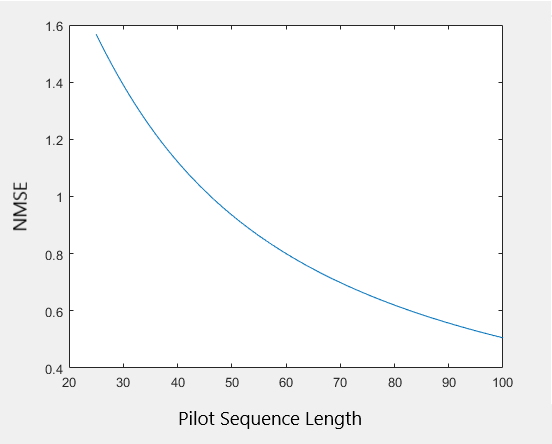
\includegraphics[width=0.45\textwidth]{MarkSchmidt-LASSO-absMSEvsPilotCount-2.PNG}}
    \subfigure[]{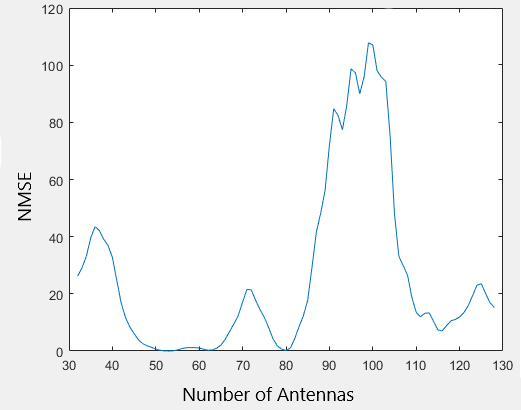
\includegraphics[width=0.45\textwidth]{MarkSchmidt-LASSO-absMSEvsAntennaCount.PNG}} 
    \caption{Results from LASSO Channel Reconstruction (a) NMSE vs. Pilot Count (b) NMSE vs. Antenna Count}
    \label{fig:lasso}
\end{figure}

Figure \ref{fig:lasso} displays the results from our MATLAB implementation of the LASSO channel estimation technique. The figures plot the NMSE versus the independent MIMO parameters, number of pilot symbols and number of antennas in a ULA. As expected, as the number of pilot symbols increases in the reference signal, the error of our estimated channel vector decreases at an exponential rate. This affirms the belief that the accuracy of the channel vector is directly proportional to the number of pilot symbols used in the reference signal sent to a UE in downlink channel reconstruction. The second image of Figure \ref{fig:lasso} shows the NMSE versus the number of antennas in a ULA. The function of number of antennas to the strength of channel estimation using the LASSO technique does not fit a common or known function. It provides an interesting insight into how the number of antennas may affect the accuracy of the LASSO technique for sparse channels. There are several peaks in the function between 30 to 50, 65 to 80, and 80 to 110 antennas. Each peak region represents ranges of antennas which produce poor channel vector estimations while using the LASSO technique. The minimum points are probably the areas of most interest as they provide insight into how many antennas are reasonable to maintain a low error of the estimated channel vector. m-MIMO systems that use LASSO channel reconstruction and have a number of antennas between 50 and 65, or 80 produce the best estimations of the channel vector. The second image used a static 50 pilot symbols to produce the following plot.

\begin{figure}[H]
\centering
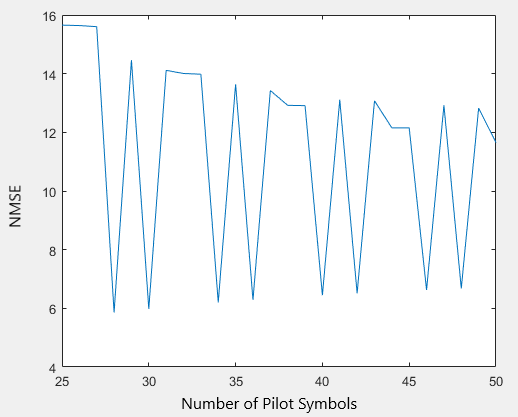
\includegraphics[width=0.5\textwidth]{figures/StackEx-LASSO-absMSEvsPilotCount.PNG}
\caption{Results from LASSO Channel Reconstruction using first method}
\label{fig:lasso-wrong}
\end{figure}

As discussed above, the first method of rearranging the complex values of the LASSO optimization problem into a real valued problem and then using MATLAB's default LASSO algorithm does not produce the expected results. Figure \ref{fig:lasso-wrong} displays the results for the NMSE versus the number of pilot symbols in the transmitted reference signals. As one can observe, the NMSE decreases irregularly as the number of pilot symbols increases. The function is quite sporadic and the does not produce results consistent with other publications \cite{Liu2016}. Therefore, this method is disregarded as it is believed something is missing or has gone wrong in the algorithm.

\subsection{Discussion}

The first method for a complex LASSO algorithm described above failed in a few different ways and can't be used as a LASSO channel sounding technique because of the large NMSE error and inconsistent results with other published works for the same technique. This leads the authors to believe that there is an implementation issue for the first method and further investigation is needed to determine the cause and propose a solution. Another issue in the development of the LASSO channel sounding method was the use of MATLAB's inverse discrete fourier transform (IDFT) function. Following the angular domain representation model of m-MIMO system defined in \cite{Tse2004}, it describes the angular transformation of the spatial transmitted signal being the IDFT of the transmitted signal, but the IDFT function in MATLAB yields results that differ from the interpretation of the textbook's. Using the unitary matrices defined in \cite{Tse2004} produce good results, while using MATLAB's IDFT produce poor results.

As shown in Figure \ref{fig:lasso}b, the number of antennas seems to affect the error of the LASSO channel sounding technique and produces an interesting function. Further research into this phenomenon should be conducted to ensure that channel sounding techniques are using the optimal number of pilot symbols and antennas in m-MIMO design so that they can preform with minimum error.

There are several variations of LASSO regression for channel sounding that take advantage of several different channel characteristics and that can be exploited to increase the accuracy and run-time speed of channel sounding. An example of another variation is the joint-burst LASSO method presented in \cite{Liu2016} which takes advantage of the burst-sparsity of the channel vector and simplifies the problem by applying a block lifting transform to the channel vector. This increases the sparsity of the channel vector and avoids issues with overlapping between bursts. The joint-burst LASSO techniques also is used for channel sounding between a BS and multiple users where the users may share joint channel vector elements \cite{Liu2016}. It makes the assumption that the number of antennas is greater than the number of users, so BSs with high traffic will need to have a large number of antennas to continue to use such a method.

The LASSO channel sounding techniques explored in this project rely on certain assumptions that may not always be valid. The uniformity of the burst-sparse signals are a key requirement for burst and joint-burst LASSO methods, but the non-uniformity of burst-sparse signals is something that should be taken into account in channel sounding techniques to ensure high precision of channel vectors in dynamic environments. Papers such as \cite{Dai2019} explore the use of machine learning and/or statistical models for modelling the non-uniformity of burst-sparse signals.

\section{Image Generation} \label{image-gen}
The images were generated using the received pilots \textit{y(n)}, or in matrix form, simply  \textit{\textbf{Y}}, following the method described in \cite{Li2020}. The code to generate the images is stored in "YOLOImageGen.m" \cite{git}. After each simulated channel the following transform would be used. 

\[
    \bar{\textbf{Y}} = \textbf{U}_{\theta}^{T}  \textbf{Y} \textbf{U}_{\tau}
\]

\noindent 
Where \(\textbf{U}_{\theta}\) and \(\textbf{U}_{\tau}\) are DFT matrices with the dimensions \([\alpha \textbf{M} \text{ x } \textbf{M}]\) and \([\beta \textbf{N} \text{ x } \textbf{N}]\) respectively; where \(\alpha\) and \(\beta\) are oversampling factors. The resulting \(\bar{\textbf{Y}}\) is a delay-angle space representation of the received pilots. The oversampling factors can be used to scale up the resolution of the images, \(\bar{\textbf{Y}}\) has the dimensions \([\alpha \textbf{M} \text{ x } \beta \textbf{N}]\). Before it is displayed the \(\bar{\textbf{Y}}\) matrix is normalized as follows. 

\[
    \Tilde{\textbf{Y}} = \dfrac{\delta}{max(|\bar{\textbf{Y}}|)} |\bar{\textbf{Y}}|
\] 

\noindent 
The resulting matrix \(\Tilde{\textbf{Y}}\) has the magnitude of \(\bar{\textbf{Y}}\) scaled between 0 and \(\delta\). The new maximum value \(\delta\) scales the brightness of the points in the resulting image. With more time it would be interesting to explore how different normalization techniques would effect the generated images with different SNR ratios. The images are generated by simply displaying the  \(\Tilde{\textbf{Y}}\) matrix. The resulting images will be gray scale and show sparsity due to the number of antennas vastly out numbering the paths. Figure \ref{fig:labeledCh} shows one of the generated images with the axis labeled.
\begin{figure}[H]
\centering
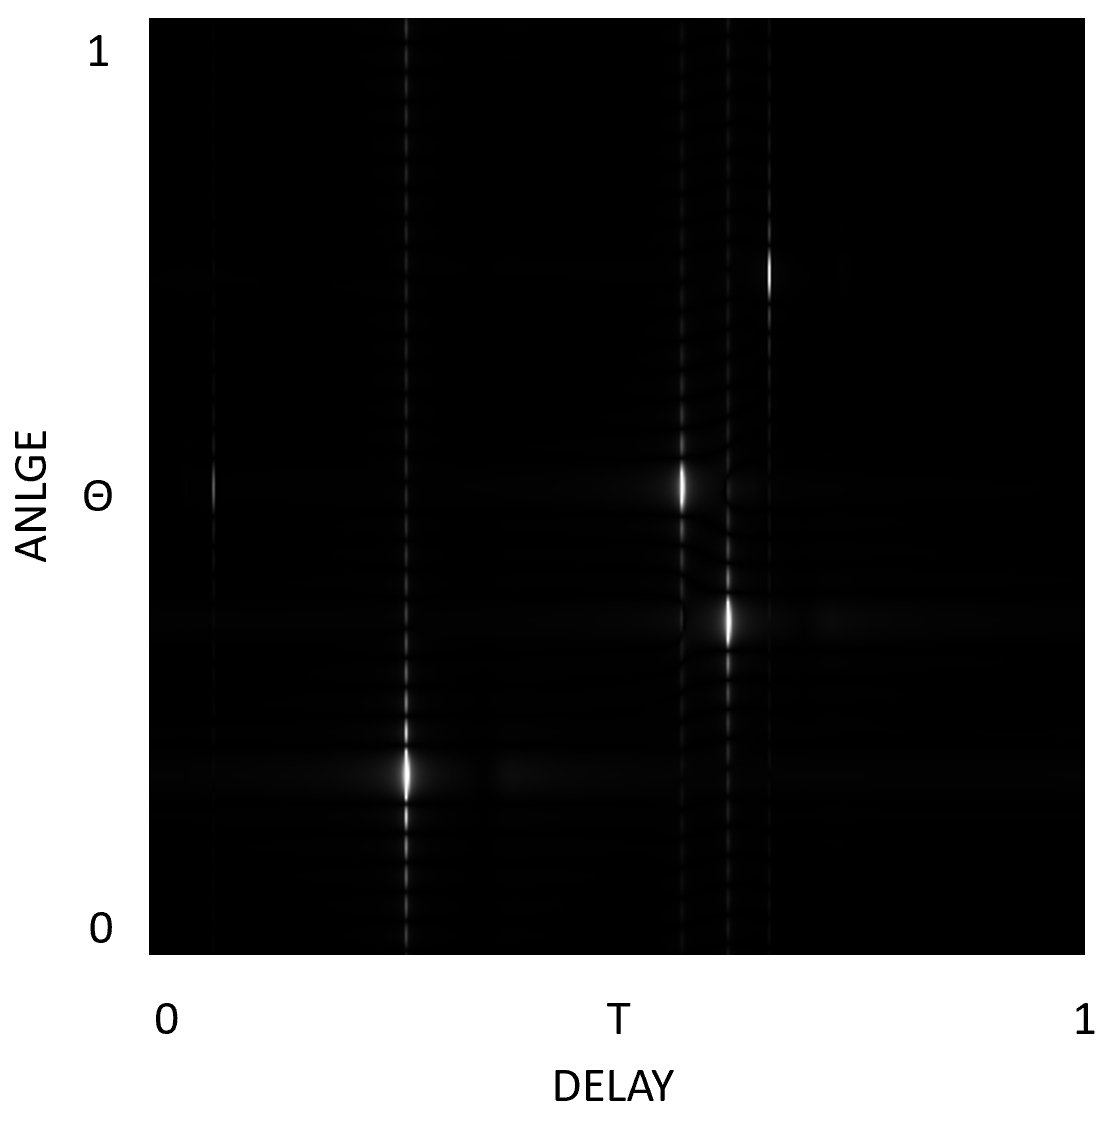
\includegraphics[width=0.5\textwidth]{figures/SYSC5804_Labeled_ChImage.png}
\caption{Labeled Channel Image}
\label{fig:labeledCh}
\end{figure}
\noindent
Each of the bright spots in the image represents a path. The coordinates of a spot are related to the antenna steering vector \(\Theta\) for the given path and the delay related phase vector \(T\). The relationship between the image and the values is shown below.

\[
    \Theta_{l} = \dfrac{y_{l}}{max(y)} - 1 
        \quad\text{and}\quad 
    T_{l} = \dfrac{y_{l}}{max(x)}
\]

\noindent 
Where \(\Theta_{l}\) and \(T_{l}\) are the value for the \(l^{th}\) path. The (\(x_{l}\), \(y_{l}\)) are the coordinates for the center point of the spot generated by the \(l^{th}\) path and (\(max(x)\), \(max(y)\)) are the width and height of the image respectively. The steering vector is subtracted by one since the image indexing starts in the top left corner. These values can be used to calculate the received angles \(\theta_{l}\) and paths delay \(\tau_{l}\) using the following equations.

\[
    \Theta_{l} =  \dfrac{d}{\lambda}\mathrm{sin}(\theta_{l})\
        \quad\text{and}\quad 
    T_{l} = \Delta f \tau_{l}
\]

\noindent
Where \(d\) is the distance between the received antennas, \(\lambda\) is the carrier wavelength, and \(\Delta f\) is the sub-carrier spacing. The \(\theta_{l}\) and $\tau_{l}$ values can be used to reconstruct the channel following the equations in Section \ref{sssec:chrec}, as is done in \cite{Han2019} and \cite{Li2020}. Unfortunately, using these equations in practice would not yield the correct path gains and delays. No matter how it was done, we could not generate the path values from the point in the image. This was disappointing, since it prevented us from closing the loop and going from received pilots all the way to a reconstructed channel.  

Varying channel conditions result in different images. Namely, changing the angle and delay of the paths changes the location of the spots in the image. Additionally, the gain of the paths is related to the brightness of the points. The SNR will also affect the image, with the noise appearing as static, the effects of varying degrees of SNR can be seen in  figure \ref{fig:snrImage}. As the SNR decreases the points become harder to recognize from the static in the background. The goal for using advanced image detection methods such as YOLO would be able to identify points in images with a lot of noise, such as figure \ref{fig:snrImage} (c). Since the image used is the normalized \(\Tilde{\textbf{Y}}\), assuming a good SNR, the dominant path is always the brightest point in the image. Other strong paths may appear dull in comparison, even if they are viable paths to transmit a signal. This can be seen in figure \ref{fig:snrImage} (a), where the LOS path is bright in the top center of the image, and another viable path is quite dim in the lower-middle right of the image. In future work we will investigate other normalization techniques to ensure the dominant path does not hide other potential paths in the image. 

\begin{figure}[H]
    \subfigure[]{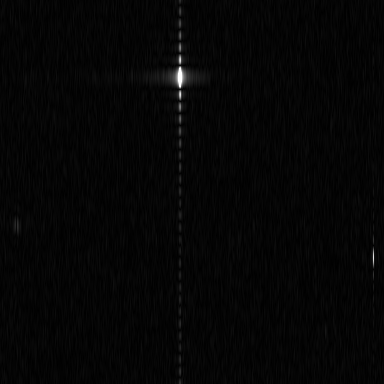
\includegraphics[width=0.245\textwidth]{SYSC5804_noNoise.png}} 
    \subfigure[]{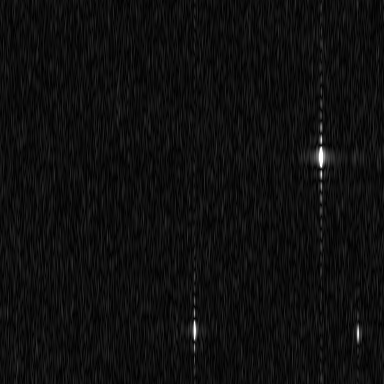
\includegraphics[width=0.245\textwidth]{SYSC5804_someNoise.png}} 
    \subfigure[]{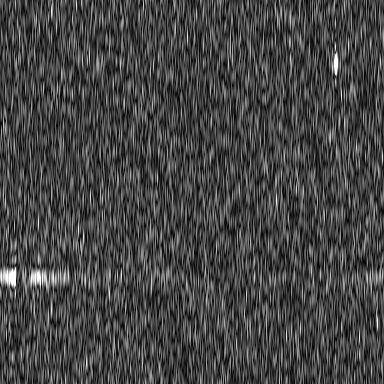
\includegraphics[width=0.245\textwidth]{SYSC5804_moreNoise.png}}
    \subfigure[]{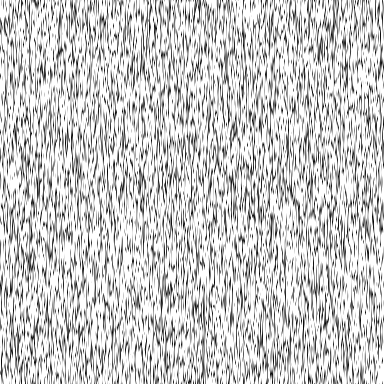
\includegraphics[width=0.245\textwidth]{SYSC5804_allNoise.png}}
    \caption{Genarated Channel Images with (a) No Noise (b) High SNR (c) Low SNR (d) Very Low SNR}
    \label{fig:snrImage}
\end{figure}



\section{YOLO} \label{yolo-main}

\subsection{Method and Implementation}

Once the channel images have been generated by using the received channel measurements as described in Section \ref{image-gen}, the spots or 'stars' within the images need to be located for channel reconstruction. This is done using the fast object detection model YOLO to identify bounding boxes for each of the spots in the images. Before using YOLO to detect the target objects within our channel images, a YOLO model needs to be trained with labelled data, so the Darknet-53 learning model can adapt to a new application. This type of learning is called transfer learning as a previously trained network is used and re-trained at a lower cost than training a network with fresh weights \cite{Burkov2019}.

Before we can train our object detection model, a training, validation, and test set of labelled data need to be generated. Many images can be generated using the image generation technique discussed in Section \ref{image-gen}, but to label the images require manual assignment of bounding boxes around the spots in the channel images. This process can be very slow, especially if the number of paths/spots or noise in the image is high. To label the bounding boxes of the spots in the image, MATLAB's Image Labeler was used to manually draw the bounding boxes for several hundred images. These images and their ground truth data are provided to the YOLO training algorithm in MATLAB to produce a detector of the white spots in the grayscale images produced by the image generator.

YOLO's network structure is described in YOLO subsection in Section \ref{background}. The image input size for the input layer of the neural network is $256 \times 256$ pixels with three colour channels. The images generated for channel estimation in Section \ref{image-gen} are $1536 \times 1536$ grayscale images which mean that the images only contain one colour channel and do not meet the requirements for the input layer of YOLO. Therefore, before the training images and bounding boxes are inserted into the trainer, the training and validation images need to be preprocessed to transform their size to the input size and add two more colour channels for full RGB capability. The preprocessing of the images used for training and validation occur before executing the training process. After training has completed, images that would like to be searched by the detector model will have to reformat themselves, as in the preprocessing steps, to extract the target objects from the images and meet the network's input requirements. As for the middle hidden layers, YOLOv3 uses the Darknet-53 network model for object detection. As our detection objects are quite simple, black background with white spots, all 53 convolution layers are not needed to preform the object detection to an acceptable degree. The convolution layer depth of the network can be set as a hyperparameter and modified in an attempt to produce a detector with the highest precision. In the case of this project, after training multiple different layer length neural networks, it was determined that the weighted Darknet-53 network would produce sufficient results when using up to the $33^{rd}$ convolution layer. The layers after that point are removed and replaced with the final transform and output layers. The transform and output layers are attached to the end of the network at the convolution layer 33 and convert the values from the network to functional predictions of the locations of spots within the channel image.

Now that the labelled training data has been collected and the network structure has been finalized, the training of the DNN can begin. The training options specified in MATLAB's training algorithms can be varied depending on the application. For the following project the YOLO network was trained on a Nvidia GTX 1060 3GB which has a small amount of VRAM and therefore cannot process large amounts of data in the Mini-batches of the Stochastic Gradient Descent with Momentum (SDGM) training technique for deep neural networks \cite{Burkov2019, Matlab2021a}. Due to the aforementioned resource restriction in VRAM, the Mini-batch size was set to 6. A maximum of 20 epochs are used during training to set a reasonable end to training a pre-trained network.

\subsection{Results}

\begin{figure}[H]
\centering
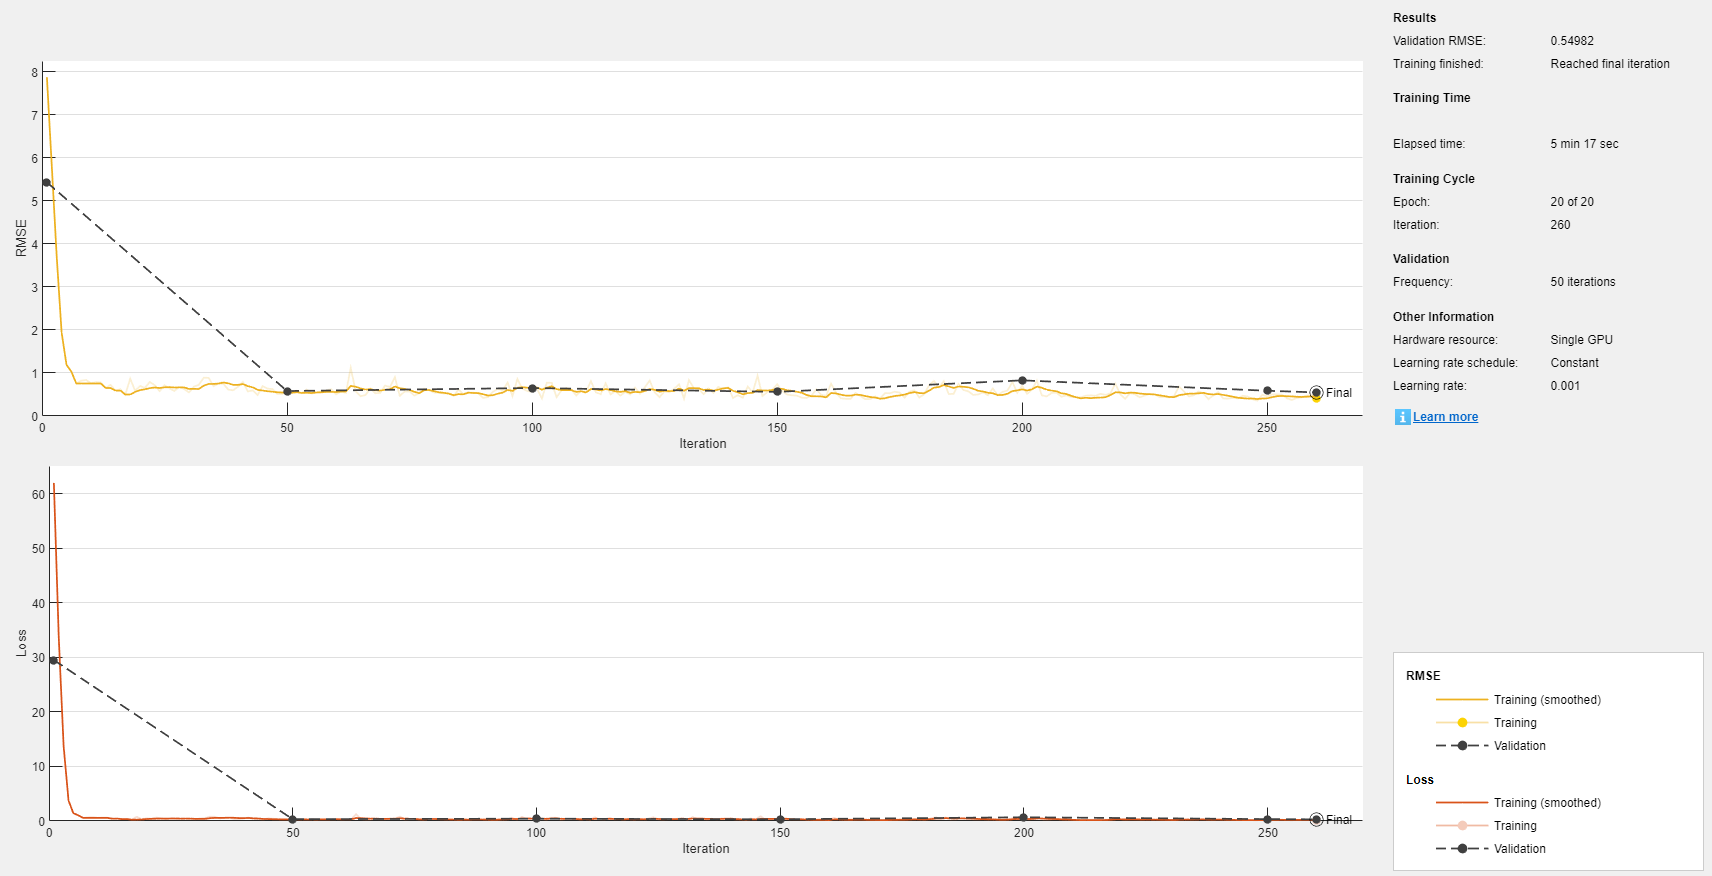
\includegraphics[width=0.9\textwidth]{figures/YOLOv3-training-2-weights-conv30.PNG}
\caption{The progression of training the YOLO model using SGDM}
\label{fig:yolo-training}
\end{figure}

Figure \ref{fig:yolo-training} shows the training progress of one of the trained detectors for the project. The top chart shows the Root Mean Squared Error (RMSE) of the model over each Mini-batch iteration with the dotted line representing the RMSE for the validation dataset. The bottom chart shows the loss over each of the iteration during training with the dotted line representing the loss of the validation set every 50 iterations. The two charts form the classic elbow shape of machine learning models using SGDM for their training as it quickly falls into a local minimum and then searches for further minimums in subsequent iterations with marginal changes. The training progress charts are updated live with the training progress in MATLAB and are very handy in monitoring and debugging the network and tuning the hyperparameters of the model.

\begin{figure}[H]
    \subfigure[]{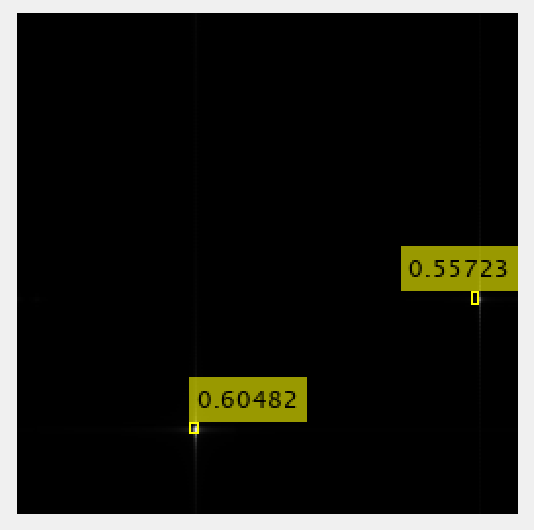
\includegraphics[width=0.3\textwidth]{CaptureExample2.PNG}}
    \subfigure[]{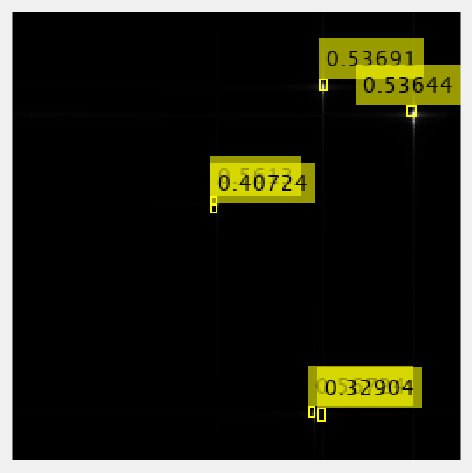
\includegraphics[width=0.3\textwidth]{CaptureExample.PNG}}
    \subfigure[]{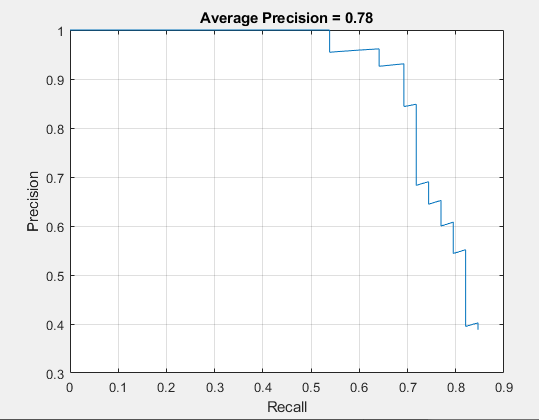
\includegraphics[width=0.38\textwidth]{YOLOv3-PRC-threshold0-25-conv30.PNG}} 
    \caption{Examples of object detection using the trained YOLO model}
    \label{fig:yolo}
\end{figure}

After the YOLO object detection model has been trained using the labelled data, testing data can be used to predict the average precision and generate plots such as the Precision-Recall Curve to evaluate the precision and recall of our detector. The Precision-Recall Curve can then be used to tune the threshold of the detector. In figure \ref{fig:yolo}c, the threshold is set to 0.25, where the threshold represents the probability that a prediction must be greater than or equal to, to be considered as a target object and returned in the detection of the model. The Precision-Recall Curve is used to evaluate the positive rate of the minority class \cite{Burkov2019}. In channel reconstruction it is important for the precision to be high, so the detector does not find false paths in the channel matrix. The recall should also be high so paths are not missed in detection. Balancing these two metrics can be difficult when tuning the machine learning model, but the Precision-Recall Curve aid in a understanding of how the model moves with respect to changes of the hyperparameters, such as threshold.

Figure \ref{fig:yolo} (a) and (b) provide examples of the detection of spots or paths within the channel image. A lower threshold is used so that fainter path components can be picked up by the detector, but many of the detected spots are detected without difficulty.

\subsection{Discussion}

Our project uses Matlab's 2021a Computer Vision, Deep Learning, and Image Processing modules which supposedly include a YOLOv2 and YOLOv3 implementation and their backing networks (Darknet-19 and Darknet-53) \cite{Matlab2021a,Matlab2021b}. During the implementation of YOLO in our project the work from \cite{Li2020,Matlab2021a,Matlab2021b} were used to construct the defined YOLOv3 for the path detection in the generated channel images. To our surprise, although the documentation was available for the YOLOv3 network, the actual network and appropriate functions defined in the documentation were not available in the latest release of MATLAB (2021a). YOLOv3's Darknet-53 network structure is available in MATLAB's deep network designer and could be installed separately to the other deep learning functions in the Deep Learning Module. Therefore, previous YOLOv2 input, transform, and output layers could be used with the Darknet-53 structure to create the YOLOv3 network without the functions described in \cite{Matlab2021b}.

When initially labelling the spots in the images for object detection, the authors drew the bounding boxes too small around the spots. This lead to a difficulty of predicting the bounding boxes for unlabelled data. This is believed to be so since the images are preprocessed and shrunk to fit the image size requirements of the input layer of the YOLO network. Small labelled bounding boxes would be transformed into small boxes with little area within and thus making the learning process for the detector more challenging. To overcome this issue, the authors were more relaxed on the bounds of the boxes around the spots in the image and the precision of the model saw a large jump.

To improve the precision of the object detection model, more labelled data should be generated. This would increase available labelled data for the training of current and future deep learning methods that use the channel image for path extraction and channel reconstruction. Most of the labelled data also contains little to no noise at all in the image, so the current detector performs poorly when attempting to identify spots in a noisy channel. This can't be the case in an actual m-MIMO system because the noise levels vary over time and space and must be accounted for in the machine learning model.

\section{AutoKeras and DNN} \label{autodnn}
Calculating the path delays and angles from labeled points was not done within the time constraints of the course, which inspired this new approach. Specifically, the problem was translating the (x,y) coordinates to the correct path angle and delay. As a work around the authors tried using a DNN to go directly from the images to the path components, completely skipping the object detection, coordinate translation, and path calculations. In essence, the idea was to brute force a solution using DNN. The model built was an image regression model, taking each of the generated images and trying to predict the path gains and delays. Some modifications had to be made, for instance the path components had to be normalized since they all had different scales. Additionally, the paths had to be sorted in the output, so the model knew which paths corresponded to the brightest points. Since it is known the path information is encoded in the image, the theory is that the right DNN would be able to extract it and calculate the path components. However, this effort was in vain, as the DNN did not predict the paths with enough accuracy. When the DNN was unable to solve the problem it was simplified to show a proof of concept. The noise was removed from the channel and the number of paths was set to be constant. 

The model was built using Autokeras, which is a DNN framework that uses Keras from Tensorflow. Autokeras is a tool to automatically generate and validate Keras models. The library treats the depth and width of the DNN's hidden layers as a hyper-parameter and optimizes the DNN structure accordingly. Initially, the models were trained locally, configured to run on a 4GB GTX1650 with Tensorflow 2.4, CUDA 11.0 and CuDNN 8.4. Despite the efforts to configure Tensorflow to train on the GPU, this still proved to be quite slow for training and testing many DNNs with a large data set. To reduce the training time the ML was moved to Google Colab; which offered a free virtual machine with a good GPU. Often Colab provided a 16GB Tesla V100 GPU. There were some limitations with Colab such as the session time and virtual storage. Autokeras stores many DNN while training with many different checkpoint versions. This quickly filled the storage on colab, limiting the amount of data used to train the network. Additionally, the Colab session would timeout and the data stored locally would be lost. 

The first model was trained using 5000 different simulated channels, with 5 different DNN's tested with a maximum epoch count of 1000. The training process took 20 hours running on Google Colab. The best model of the 5 barely predicted values better then random. The data was normalized to be in the range of 0 to 1, using a 'min\_max\_scalar' from sklearn. The model was trained to predict the path angles and delays. The resulting RMSE was 0.3, which was not much better then predicting random values. Figure \ref{fig:dnnres} shows the predicted values plotted against the true values for the path delays and angles of the first path.
\begin{figure}[H]
    \subfigure[]{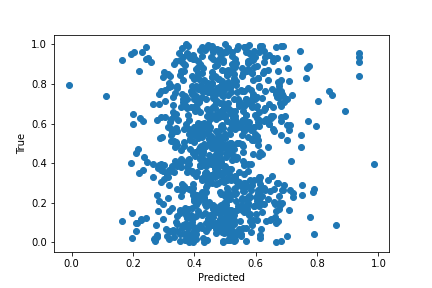
\includegraphics[width=0.45\textwidth]{T_1.png}} 
    \subfigure[]{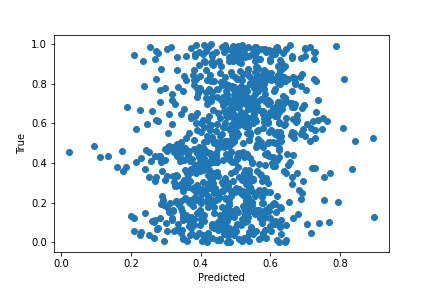
\includegraphics[width=0.45\textwidth]{AoA_1.png}}
    \caption{Predicted vs True Values for Path 1's (a) Delay (b) Angle}
    \label{fig:dnnres}
\end{figure}
\noindent
It is clear when looking at these results the predictions are all normally distributed around the mean and do not correlate with the true values. The better the predicted values, the closer they would be to the \(y=x\) line.

The first attempt seemed fundamentally flawed, too much time was spent training the model and not enough resources were focused on identifying the correct DNN. The second attempt used drastically less data, but tested far more DNNs. The data set consisted of 500 channel images and Autokeras trained 30 models over 100 epochs. Reviewing the results of the previous attempt the validation error was improved by an order of magnitude over epoch 101-1000. The extra hours spent training were not useful since the model did not generalize. This attempt was significantly faster, only running for 6 hours however came with a new issue. The 30 DNNs trained generated a massive amount of data to be stored (60GB+), which exceeded the storage capacity on the colab instance. This caused the virtual machine to crash, with the model unrecoverable. 

Instead of running on the server this approach was tested locally, and showed promising results. The local GPU could not support this heavy of a model, so the images were scaled down to 128 pixels\(^{2}\) from 384 pixels\(^2\); reducing the number of input nodes in the network by an order of magnitude. This increased the size of training batches significantly, reducing the training time for each epoch to tens of seconds instead of a full minute. This comes at a cost though, the resolution of the image is directly related to the accuracy of our predictions. Additionally, only the path delays were predicted to further reduce the complexity. Even with the simplification it took 10 hours to generate and train the models locally with the GTX 1650. The resulting model had a RMSE of 0.1, outperforming the previous attempt by a factor of 3; however, it was not enough to accurately reconstruct the channel. This shows the DNN architecture from this approach is far better for solving the problem then the one generated in the first approach. Figure \ref{fig:laptopT} shows the predicted vs true results for the first path. It does not look drastically better then the previous plots, however, the density around the $y=x$ is much higher, as shown by the improved RMSE. Although, had the DNN architecture generated from this approach been trained with 1000 epochs, full image resolution, and the 5000 image data set used for the previous trial, it would likely improve performance dramatically. This was be the next step for the DNN approach, however due to the massive amount of time to test these models it was not completed in time for the report submission.

\begin{figure}[H]
    \centering
    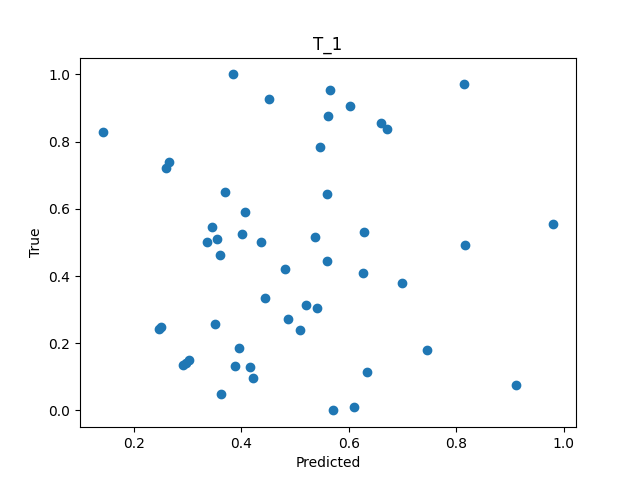
\includegraphics[width=0.49\textwidth]{figures/T_1_laptop.png}
    \caption{Laptop Predictions with Drastically Less Resources}
    \label{fig:laptopT}
\end{figure}



\section{Conclusion}
This paper documents the authors' term project for SYSC5804: exploring channel reconstruction for m-MIMO systems. The study was based on NR communication systems simulated using MATLAB's 5G Toolbox. State-of-the-art channel reconstruction techniques were recreated in MATLAB and Python; methods include LASSO regression based approach \cite{Liu2016} and a YOLO image processing technique \cite{Li2020}. Additionally, the authors experimented with new methods, such as applying Deep Neural Network directly to the received pilots to predict the path gains, angles, and delays. This is an active research area for 5G systems that is both computationally and analytically complex. Some challenges arose that were not overcome within the time constraints of the course; however, there were many interesting results generated and the directions explored showed potential. The authors plan to continue this work in the future and hope to pursue a publication in the space. The remainder of this section will highlight the novel contributions from this work and the next steps for this research. Any feedback or suggestions for future work would be greatly appreciated! 

\subsection{Contributions}
Although this work was mostly focused on recreating stat-of-the-art channel reconstruction techniques there were several interesting contributions. Firstly, all the code for the channel simulator and the channel reconstruction algorithms implemented is freely available with documentation on GitHub \cite{git}. Prior work in this space has always kept the source code proprietary. Our project could act as the building blocks for future research in this space. The channel image generation algorithm is available, along with sample data sets that include the ground truth data for the paths. Additionally, several of these data sets have included YOLO bounding box labels validated manually, as well as pre-trained YOLO weights. Additionally, the antenna based analysis of LASSO performance was novel. Prior researchers had not shown how LASSO performance was affected by antennas count. Studying the ideal antenna configurations for LASSO regression analysis could be valuable future research.  

\subsection{Future Work} 

The authors believe there is potential to use DNNs to improve the state-of-the-art image based path recognition from the received pilots. First, it would be interesting to explore how DNN image processing methods compared to classical methods such as LASSO in low SNR scenarios. A full analysis and performance comparison between the two techniques would generate worthwhile results. Additionally, \cite{Li2020} uses YOLO to detect points in the image, it would be interesting to apply DNNs to the problem directly. This was already investigated as part of the project, without results. This is largely due to how resource intensive State-of-the-art deep learning solutions are. With more time and some better resources we believe models can be made to go directly from received pilots in either time-antenna or delay-phase space to the path components. Furthermore, there was a thought to explore using DNNs to solve the implementation problem in the YOLO method. Instead of mathematically going from the pixel coordinates to the path delays and angles, a DNN could predict these values. It may not be as effiecent, although it would be interesting to see if the algorithm could solve the math problems that we could not.

Classical image processing techniques may improve path detection. There are likely faster algorithms for high SNR scenarios, since the paths are more obvious. It would be interesting to study using classical computer vision techniques and a hybrid technique that combines classical object detection with deep learning \cite{mahony2019}. For instance, performing a convolution on the image with a sharpening matrix will make the faint paths far more apparent, simplifying their extraction from the image. Another interesting approach would be applying a threshold, changing all pixels under it to black and over it to white. This threshold can be scaled up or down until there is a desired number of paths in the image. This is shown in figure \ref{fig:thld}, where the paths are far clearer in the image after applying the threshold. 

\begin{figure}[H]
    \subfigure[]{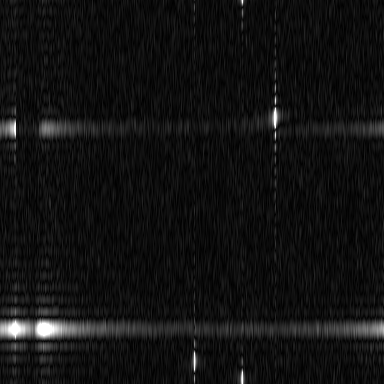
\includegraphics[width=0.49\textwidth]{91.png}} 
    \subfigure[]{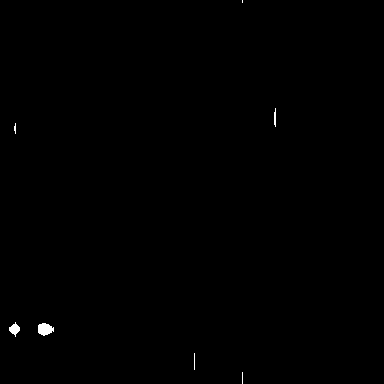
\includegraphics[width=0.49\textwidth]{figures/91_threshold.png}}
    \caption{Threshold Example (a) Original Image (b) After Applying Threshold}
    \label{fig:thld}
\end{figure}
\noindent

Finally, we are interested in exploring how these algorithms will expand to other antenna array configurations. All the novel m-MIMO channel reconstruction techniques use uniform linear arrays of antennas to simplify the model. This is good for a proof of concept; however, it is not a practical assumption, as any m-MIMO deployed will not have all its antennas in a single line. Supporting more complex antennas arrays will require extrapolating the math into higher dimension, since a single angle will not fully represent the path. A deeper understanding of antenna configurations and the channel reconstruction math is required before we can explore this avenue.

\newpage
\bibliographystyle{./bibliography/IEEEtran}
\bibliography{./bibliography/IEEEabrv,references}


\end{document}
